\documentclass{article}
\usepackage[utf8]{inputenc}
\usepackage[spanish]{babel}
\usepackage{listings}
\usepackage{graphicx}
\graphicspath{ {./images/} }
\usepackage{cite}
\usepackage{wrapfig}

\begin{document}

\begin{titlepage}
    \begin{center}
        \vspace*{1cm}
            
        \Huge
        \textbf{Informe De Implementacion}
            
        \vspace{0.5cm}
        \LARGE
        Parcial 2
            
        \vspace{1.5cm}
            
        \textbf{Manuela Gutiérrez Rodríguez}
        \vspace{0.5cm}
        
        \textbf{Daniela Andrea Gallego Díaz}
            
        \vfill
            
        \vspace{0.8cm}
            
        \Large
        Despartamento de Ingeniería Electrónica y Telecomunicaciones\\
        Universidad de Antioquia\\
        Medellín\\
        26 de Septiembre de 2021
            
    \end{center}
\end{titlepage}

\tableofcontents
\newpage
\section{Clases implementadas}

Entre las clases que implementamos para la solucion de este problema fueron:

\subsection{Función submuestreo: }
Esta clase cuenta con dos atributos, el primero es un vector llamado matrizRGB que se encarga de almacenar los valores relacionados al RED, GREEN Y BLUE  que contiene cada pixel de la imagen leida; el segundo atributo es un vector de vectores llamado matrizPixeles que se encarga de almacenar el valor medio de un grupo de pixeles, guardando en cada una de sus posiciones un vector que contiene valores de RED, GREEN Y BLUE. A su vez, esta clase cuenta con cuatro métodos, el primero que es su constructor por defecto que recibe como parámetro de entrada una imagen de tipo QImage, en el constructor se realiza todo el proceso de submuestreo que se almacena en matrizPixeles, su segundo método es una sobrecarga del constructor que recibe una imagen de tipo QImage y un entero que indica el método a utilizar, este constructor solo se utiliza cuando la imagen necesita submuestreo en una única dimensión, al igual que el anterior constructor almacena los pixeles luego del submuestreo en matrizPixeles, su tercer método llamado GuardarTxt se encarga de almacenar los valores de matrizPixeles en un formato específico en un archivo .txt para comodidad del usuario a la hora de trasladar estos valores a la plataforma tinkercad, el cuarto y último método consiste en una función que va a permitir retornar el contenido de matrizPixeles.

\subsection{Funcion sobremuestreo:}
En esta funcion se implementan tres metodos, el constructor por defecto el cual tiene la funcion de recibir la ruta escrita por el usuario y almacenarla en un atributo privado de la clase para asi poder leer la imagen. Tambien un metodo llamdo lectura, que se encarga de leer cada pixel de la imagen de acuerdo al RGB y almacena cada valor en un vector de vectores (atributos privados de la clase), uno para los pixeles rojos, otro para los verdes y por ultimo los azules. El ultimo metodo implementado fue el de redimension, alli se hace el proceso de redimension de la imagen donde se itera sobre las matrices RGB y se van añadiendo pixeles teniendo encuenta las dimensiones originales y cuantos pixeles se deben agregar para llegar a una matriz de 12x12, en este mismo metodo almacenamos la matriz final ya redimensionada en un archivo .txt para asi utilizarlo como recurso para la implementacion en la plataforma de Tinkercard.


\section{Esquema de clases implementadas}
\subsection{Función submuestreo: }

\begin{itemize}
\item Atributos privados de la clase:

\hspace{0.5cm}Vector matrizRGB

\hspace{0.5cm}Vector de vectores matrizPixeles

\item Metodos de la clase:

\hspace{0.5cm}Submuestreo(QImage): permite tomar el valor medio de un conjunto de pixeles, determinado por el tamaño de la imagen y como ésta debe dividirse para encajar en la matriz de leds de 12x12. El proceso que se realiza parte desde el origen y toma un punto aledaño en el eje y y en el eje x, para hallar el pixel que se encuentra en medio de estos 3, de esta forma se reduce la cantidad de pixeles que tiene la imagen. 

\hspace{0.5cm}Submuestreo(QImage,int): según el tamaño de la imagen permite redimensionarla en el eje x o y, hallando el valor del pixel medio del dividisión del eje a submuestrear. Este proceso inicia en el origen del eje a submuestrear y toma dos puntos en este y toma el pixel que se encuentre en medio de los dos.

\hspace{0.5cm}GuardarTxt: a partir de el vector de vectores matrizPixeles, almacena sus valores en un formato adecuado para copiar el contenido almacenado en el archivo ImagenPixeles y pegarlo adecuadamente en tinkercad.

\hspace{0.5cm}getMatrizPixeles: retorna el vector matrizPixeles.


\end{itemize}

\subsection{Funcion sobremuestreo:}
\begin{itemize}
\item Atributos privados de la clase:

\hspace{0.5cm}Variable string llamada ruta (almacena la ruta donde se encuentra la imagen seleccionada por el usuario)

\hspace{0.5cm}Un vector que contiene vectores, estos contienen las matrices segun el RGB (tres matrices en total por cada color)

\item Metodos de la clase:

\hspace{0.5cm}Sobremuestreo: Constructor por defecto, recibe un string el cual le da al atributo ruta la direccion que escribe el usuario, donde se encuentra la imagen a procesar.

\hspace{0.5cm}Lectura: Metodo que lee la imagen y almacena los valores de cada pixel en vectores que contienen vectores, cada uno segun el RGB.

\hspace{0.5cm}Redimension:Metodo que itera sobre cada una de las matrices RGB y va almacenando y agregando pixeles de acuerdo a las dimensiones de la imagen original para asi, en un archivo .txt tener todos los valores correspondientes con dimension 12x12.


\end{itemize}

\section{Modulos de codigo}


\begin{itemize}
\item Interacción de la clase QImage con la clase submuestreo y sobremuestreo:

\hspace{0.5cm}QImage imagen(ruta.c_str());

\hspace{1.5cm}if(imagen.width()<12 and imagen.height()<12){ --relacion del tamaño de la imagen con el método a implementar
    
\hspace{2cm}Sobremuestreo uno(ruta); --implementación sobremuetsreo
        
\hspace{2cm}uno.Lectura();
        
\hspace{2cm}uno.Redimension();
        
\hspace{0.5cm}}
    
\hspace{1.5cm}else if((imagen.width()>=12 and imagen.height()>=12)){
    
\hspace{2cm}Submuestreo dos(imagen); --implementacion submuestreo
        
\hspace{2cm}dos.GuardarTxt();
        
\hspace{1.5cm}}

\item Interacción de la clase qImage con la clase submuestreo:

\hspace{0.5cm}anchoProm=imagen.width()/12; --tamaño en x en la que se debe dividir la imagen, se usa el método width() de la clase qImage

\hspace{0.5cm}altoProm=imagen.height()/12; --tamaño en y en la que se debe dividir la imagen, se usa el método height() de la clase qImage

\hspace{0.5cm}for(int y=0; y+altoProm<=imagen.height(); y+=altoProm){ --ciclo en relacion al alto de la imagen

\hspace{1cm}ytotal=(2*y+altoProm)/2;

\hspace{1cm}for(int x=0; x+anchoProm<=imagen.width(); x+=anchoProm){ --ciclo en relacion al ancho de la imagen

\hspace{1.5cm}xtotal=(2*x+anchoProm)/2;

\hspace{1.5cm}matrizRGB.push_back(imagen.pixelColor(xtotal,ytotal).red());
--método de la clase 

QImage para obtener el valor en RED

\hspace{1.5cm}matrizRGB.push_back(imagen.pixelColor(xtotal,ytotal).green()); --método de la clase QImage para obtener el valor en GREEN

\hspace{1.5cm}matrizRGB.push_back(imagen.pixelColor(xtotal,ytotal).blue());
--método de la clase 

QImage para obtener el valor en BLUE

\hspace{1.5cm}matrizPixeles.push_back(matrizRGB);

\hspace{1.5cm}matrizRGB.clear();

\hspace{1cm}}

\hspace{0.5cm}}


\item Interacción de la clase qImage con la clase sobremuestreo:

\hspace{0.5cm}for (int fila=0; fila<imagen.height(); fila++){ --se usa el método height() de la clase qImage

\hspace{1cm}filas=vacio;

\hspace{1cm}for(int columna=0; columna<imagen.height(); columna++){ --ciclo en relacion al alto de la imagen

\hspace{1.5cm}filas.push_back(imagen.pixelColor(columna,fila).red()); --método de la clase QImage 

para obtener el valor en RED

\hspace{1cm}}

\hspace{1cm}matrizPixelesrojos.push_back(filas);

\hspace{0.5cm}}

\hspace{0.5cm}for (int fila=0; fila<imagen.height(); fila++){ --ciclo en relacion al alto de la imagen

\hspace{1cm}filas=vacio;

\hspace{1cm}for(int columna=0; columna<imagen.height(); columna++){ --ciclo en relacion al alto de la imagen

\hspace{1.5cm}filas.push_back(imagen.pixelColor(columna,fila).green()); --método de la clase QImage 

para obtener el valor en GREEN

\hspace{1cm}}

\hspace{1cm}matrizPixelesverdes.push_back(filas);

\hspace{0.5cm}}

\hspace{0.5cm}for (int fila=0; fila<imagen.height(); fila++){ --ciclo en relacion al alto de la imagen

\hspace{1cm}filas=vacio;

\hspace{1cm}for(int columna=0; columna<imagen.height(); columna++){ --ciclo en relacion al alto de la imagen

\hspace{1.5cm}filas.push_back(imagen.pixelColor(columna,fila).blue()); --método de la clase QImage 

para obtener el valor en BLUE

\hspace{1cm}}

\hspace{1cm}matrizPixelesazules.push_back(filas);

\hspace{0.5cm}}



\end{itemize}

\section{Estructura del circuito}

Para la construcion del circuito hemos utilizado 12 tiras de 12 leds neopixel, para asi tener una dimension de 12x12, conectados a una fuente de energía para evitar el retraso a la hora de ejecutar la simulación. La primera tira se enceuntra conectada a un pin y a través de este se envía información al resto de tiras, debido a que se encuentran conectadas las salidas con las entradas. Las conexiones de voltaje y tierra se realizaron en paralelo.

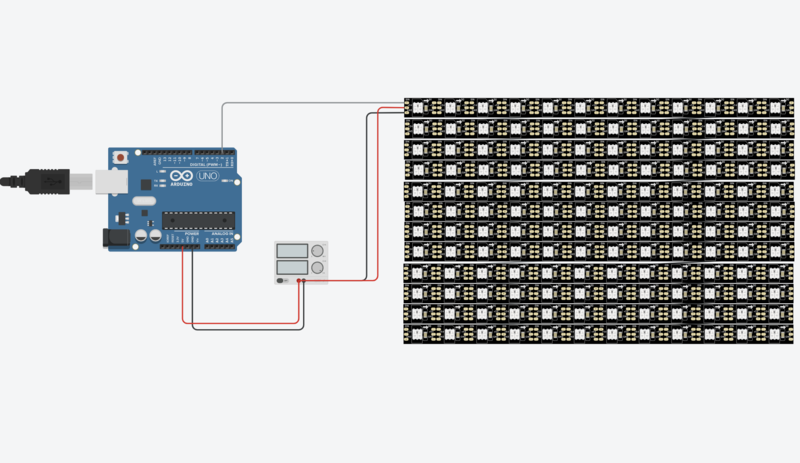
\includegraphics{images/Circuito.png}

\section{Problemas presentados}
\begin{itemize}

\item A la hora de buscar la lógica para las funciones de submuestreo y sobremuestreo, debido a que nos costaba un poco plantear el algoritmo para la redimensión.

\item Cuando se buscó la forma de crear clases relacionadas a las funciones.

\item Relacionado al repositorio, al principio nos costó entender como debíamos sincronizar los repositorios locales con los remotos, también al intentar deshacer algunos cambios.

\item Respecto a las indicaciones, ya que se preguntó si en una imagen de 18x10 se debía hacer submuestreo en una dimensión y sobremuestreo en otra, a lo cual la respuesta obtenida fue no, el último día el profesor Augusto indicó que el programa debía tener la capacidad de submuestrear y sobremuestrear este tipo de imagenes.



\end{itemize}


\end{document}
